\documentclass[runningheads,a4paper]{llncs}

\usepackage{amssymb}
\usepackage[utf8]{inputenc}
\usepackage{subfig}
\setcounter{tocdepth}{3}
\usepackage{graphicx}
\usepackage{tikz}
\usepackage{tikz-qtree}

\usepackage{url}
\usepackage{lingmacros}
\newcommand{\keywords}[1]{\par\addvspace\baselineskip
\noindent\keywordname\enspace\ignorespaces#1}

\begin{document}

%passwords to the submission: ID 467 klasse
\mainmatter  % start of an individual contribution

% first the title is needed
\title{A Type-Theoretical Wide-Coverage Computational Grammar for Swedish}

\author{}
\institute{}


\maketitle


\begin{abstract}
The work describes a wide-coverage computational grammar for Swedish. 
It is developed using GF(Grammatical Framework), a dependently-typed 
functional language, specialized for grammar programming. We trained
and evaluated the grammar by using Talbanken, one of the largest treebanks for 
Swedish. As a result 65 $\%$ of the Talbanken trees were translated
into the GF format in the training stage and 75 \% of the noun phrases
was parsed during the evaluation. Moreover, we obtained a language
model for Swedish which we use for disambiguation when parsing free text
with the grammar. 
\keywords{grammar-formalism, computational grammar, treebank}
\end{abstract}


\section{Introduction}

%Motivation + brief information about Swedish+resources.

%Introduction + Aim from Master thesis(Chapter 1 + 1.1).

%Outline of the paper. 

Two main approaches divide the research in computational linguistics
in the last years. The first one is the wide-coverage method, usually based on
statistics methods, which compensates its usually shallow analysis of the
input with its coverage. The other approach is the opposite - provides
a deep analysis of the data, but it's coverage is limited to
very specialized input. Our work tries to unite the two approaches by
developing a wide-coverage computational grammar for Swedish. We start
with a minimal model of the language and extend its coverage
significantly, without affecting the quality. The grammar was
developed and evaluated against Talbanken\cite{talbanken}, one of the
largest Swedish treebanks. 



%The paper is organized as follows: .... \textbf{maybe leave out if no space}


\section{Background}

\subsection{GF}
\label{sec:gf}

The computational grammar was developed within GF(Grammatical
Framework) \cite{gfbok}. GF is a dependently-typed grammar formalism,
based on Martin-Löf type theory, which is mainly used for
multilingual natural language applications. 

GF grammars are composed of an abstract syntax, interlingua of the
grammar, describing the semantics on a language-independent level and
a number of concrete syntaxes, usually corresponding to natural
languages. These describe how the concepts from the abstract syntax
are described in the language. 
By defining such a grammar, one also obtains a parser for the language
fragment that is described by a concrete grammar and a natural
language generation tool that is able to generate constructions from
the same language fragment. 
In this way, due to the division of the GF
grammars into abstract and concrete, it is possible to achieve 
semantics-preserving translation between any pair of languages from 
the grammar. 
 
However, because the grammar is strict, we can only deal with
constructions that the grammar defines and nothing more. One could
classify the limitations of the natural language grammar in two
categories --- missing lexical items and missing syntactic
structures. For this reasons GF was mainly used so far for controlled
languages\cite{cnl} and, dialogues systems \cite{talk} and interactive 
systems where the user is guided to stay
within the bounds of the grammar by a predictive
parser\cite{parser}, such as a multilingual tourist
phrasebook\cite{phrasebook}. 
However, there is some recent work on parsing
free text --- a grammar for patent claims from the biomedical
domain \cite{patent}. This work highlighted a
number of caveats of real-world text, but in the same time gives
valuable insights that future work on wide-coverage GF grammars can
benefit from.

The current work aims at overcoming the second limitation of GF
grammars --- adding support for the most common syntactic
constructions that could appear in Swedish texts. For some of these we
use dependent types to encode the syntactic phenomena in an elegant
way. The lexicon limitation is not a problem, as we use an existing 
large Swedish lexicon \cite{ahlbergEnache}, which is being continuously
developed and contains more than 120 000 entries.
%... \textbf{Malin, can you say a bit more ?But not more than a couple
%  of lines :)}  




\subsection{Swedish}

% Chapter 2.4(with emphasis on the syntactic structures)
Swedish is a North-Germanic language, sharing most of its grammatical structure 
with Norwegian and Danish. It is also one of the official languages in Finland
and is spoken by approximately 9 million people.
Although Swedish syntax often is similar to English, the  morphology is richer and the
word order more intricate.
It is a verb-second language: %\cite[p.116]{gunlog}: 
the second constituent of a declarative main clause must consist of a verb.
The normal word order is subject-verb-object, but fronting other constituents
-- topicalisation -- is very common,  especially for temporal and
locative adverbial phrases \cite[\textsection 1027]{H&H}.
Fronting the finite verb marks questions.
%\enumsentence{Passive \hspace{45mm} Active\\
%\shortexm{12}
%{Tjuven & togs&  av & polisen}
%{\emph{the}\emph{ thief}&  \emph{took}+\textbf{s}&  \emph{by}&\emph{the police}}
%{``The thief was arrested by the police"}
%{&&Polisen & tog & tjuven}
%{&&\emph{the police} & \emph{took} & \emph{the thief}}
%{\hspace{-9mm}``The police arrested the thief"}}
%\label{gfPass:s-pass}
Special reflexive pronouns and reflexive possessive pronouns for the 3rd
exist \cite[\textsection 310 \& 319]{H&H}, distinct from the normal 3rd person forms.
%\enumsentence{
%\begin{tabular}{llll}
%a. & Han slog \textbf{sig}.&\hspace{6mm}b. & Han såg \textbf{sitt} barn.\\
%&\emph{He hit \sc self.} && \emph{He saw {\sc self's} child.}\\
%c. &Han slog \textbf{honom}. &\hspace{6mm}d.& Han såg \textbf{hans} barn.\\
%&\emph{He hit him (another person).}&&\emph{He saw his (another person's) child.}
%\end{tabular}}






\subsection{Talbanken}

%Chapter 2.2
\label{sec:talbanken}
For testing and evaluation of the grammar and lexicon, we needed to be able to
compare them against a reliable source.
We have used Talbanken \cite{talbanken},
a freely available, manually annotated, large-scale treebank.
It is analyzed with the MAMBA annotation scheme (Teleman, 1974) and 
the more than 6000 sentences we have been using
%consists of four
%parts. Two of them are transcriptions of spoken language, one a collection of
%text written by high school students, and one, section P,
consists of professionally written Swedish gathered from newspapers, brochures and textbooks.

Talbanken was also used to train the Swedish version of the Malt parser \cite{malt}
and was then redistributed in an updated version,
Talbanken05 \cite{talbanken05}.
%It is released in Malt\footnote{http://w3.msi.vxu.se/~nivre/research/MaltXML.html} 
%and Tiger\footnote{http://www.ims.uni-stuttgart.de/projekte/TIGER/TIGERSearch/doc/html/TigerXML.html}
%XML-formats
%where the trees have been made deeper and more detailed while still containing
%the lexical MAMBA layer. 
%The Malt parser was trained on section P of Talbanken, and these
%more than 6000 sentences have been used our project. 
%The treebank has served as an inspiration and an evaluation source throughout the
%project.



 
\section{Related Work}
%\textbf{Ramona: also just copied, if you want, improve it}
%Chapter 2.5 - w/o the references about lexical resources
%
%Mention the LREC paper and what it does, without any direct reference
%between the authors
There exist a number of parser for Swedish already, such as the
data-driven Malt parser \cite{malt}, also trained on Talbanken, the 
cascaded finite state parser CassSwe \cite{casswe}, % and
The Swedish Constraint Grammar \cite{birn} and the Swedish FDG, which
uses the Functional Dependency Grammar \cite{fdg}.
%which gives syntactic analyses. \textbf{I don't really know if the
  %last 2 do... could you rephrase please ?} 

Among computational grammars for Swedish, we mention the Swedish
version of the Core Language Engine \cite{gamback}, which
provides a comprehensive description of syntax and semantics, as well
as a translation to English. Unfortunately, the resource is not
available for comparison. Other grammars are BiTSE \cite{stymne}, a
Swedish grammar that uses the HPSG format \cite{hpsg} and developed
within the LinGO Matrix library \cite{matrix}. 

The current work uses the extensive Swedish
lexicon developed in \cite{ahlbergEnache} and the Swedish resource
grammar as a starting point. 

Currently, GF is the leading technology in the European project
MOLTO (Multilingual On-Line Translation)
\footnote{http://www.molto-project.eu/}, which aims at developing
 tools for translating between 15 languages in real-time and with high quality. 

Previous examples of larger type-theoretical GF grammars that use 
dependent-types are SUMO-GF \cite{ontologies2}, a GF representation of
SUMO \cite{sumo}, the largest open-source ontology and  a natural
language generation grammar via Montague semantics \cite{montague}.



\section{Grammar}

%Discussion about the two dimensions of a grammar - lexicon and syntax 
There are two aspects of on a computational grammar -- the work on the lexicon
and the work regarding syntax.  For this article, we will focus on the
syntactical dimension of our work, the description and formalization of grammar
rules and the usage of Talbanken.

\subsection{Resource grammar}

%Chapter 2.1.2
The GF package provides an useful resource library \cite{gf-resource}, covering the
fundamental morphology and syntax of more than 20 languages.
There is also a small test lexicon included, containing a few hundred common
words.
%Since the languages all share the same abstract syntax translation between any given
%pair is possible, which is valuable
%when implementing multilingual applications.
The grammars describe how to construct phrases and sentences and how to
decline words. They cover the morphology,
word order, agreement, tense, basic conjunction etc.
Due to the syntactic similarities between the Scandinavian languages, much of
the implementation for Swedish is shared with Norwegian and Danish. The modules
that concern the lexical aspects are separate, while 85 \% of the syntax
description is shared.  There are about 80 functions, which describe the rules
for building phrases and clauses.
\begin{verbatim}
PredVP       : NP -> VP -> Cl ; -- Predication
ComplVPSlash : VPSlash  -> VP ; -- Complementation
\end{verbatim}
%The analysis preformed by GF is driven by the parts of speech, which are combined into
%parts of sentences.
In addition to the core resource grammars, which is shared with all other
languages implemented in the library, there is also an extra module
%, simple called the \verb|Extra| module,
where language specific constructions may bee added
%The functions given here do not have to be translatable
%to all other language, but are meant to cover language specific constructions.


\subsection{Lexicon}

%Everything about Saldo, Lexin, etc, compressed.
%
%We use the resources from the other paper, so to say :)
As mentioned before, our main lexical resource is SALDO \cite{saldo} from
which a GF lexicon has been extracted \cite{ahlbergEnache}.
Valency information, which is a key feature to good parsing using GF,
are extracted from the lexicon
Lexin\footnote{http://spraakbanken.gu.se/lexin/}.
This gives us a dictionary with more than 100 000 entries, covering all but 500
words from Talbanken (excluding names, compounds and numerical expressions).

\subsection{New Features}

%Section 4.2
%
%Selection of additions to the grammar 
%
%- reflexive possesive pronouns
%
%- s-passive
%
%- impersonal constructions
%
%- miscellaneous 
It has earlier been hard to identify missing constructions of the Swedish
implementation since there was no large resource available to evaluate it on.
Our evaluations are based on Talbanken and when first conducting tests
 we found much room for improvement. The items listed below are examples
 of constructions implemented during this work.\\

\noindent\textbf{The s-passive}
Swedish has two ways of forming passive verb phrases: the 
periphrastic passive, formed by using the modal auxiliary verb `bli'
(\emph{`become'})
and the s-passive which is formed by adding an \emph{s} to the verb. 
Passive voice is often used, especially the
s-passive, % (sentence \ref{gfPass:s-pass}).
which is used in more than 80 \% of the times according to some studies 
%Some studies suggest that the s-passive is 
\cite{laanemets}.
It is however not as common in the other Scandinavian languages, 
where not all words have passive forms for all tenses. The resource grammar for
Scandinavian therefore only implemented the periphrastic passive.
%\verb-PassV2-, by using auxiliary verb.
%The function allows two-place verbs to be used in passive by using \emph{bli} (\emph{become}), and thereby
%turned into complete verb phrases; they no longer need an object.
During this project, the s-passive was added although the
periphrastic passive is still allowed.
%The grammar further allows not only transitive verbs, but 
%All verb phrases that misses an object are allowed to form passives.
A ditransitive verb -- \emph{ge} (`give') (\ref{sent:give2pass}) -- gives rise to two
passives, (\ref{ex:passV33}) and (\ref{ex:passV32}), both covered by our new implementation.
\eenumsentence{
\item{\textbf{Active use of two-place verb}\\\shortex{4}
{Vi & erbjöd& henne& jobbet }
{\emph{we} & \emph{offered}& \emph{her}&\emph{the job}}
{``We offered her the job"}}
\label{sent:give2pass}
\item{\textbf{Passive use, first place \hspace{3mm}Passive use, second place}\\\shortex{7}
{Hon & erbjöds & jobbet && \hspace{3mm}Jobbet & erbjöds & henne }
{\emph{she} &\emph{ offered+\textbf{s}}&\emph{ the job}
&&  \hspace{3mm}\emph{the job} & \emph{offered+\textbf{s}}&\emph{ her}}
{``She was offered the job"}
~``The job was offered to her"}}
\label{ex:passV33}
%\item{\textbf{Second place in two-place verbs}\\\shortex{3}
%{Jobbet & erbjöds & henne }
%{``The job was offered to her"}}
\label{ex:passV32}}


\subsubsection{Impersonal constructions}
\label{sec:Formal}
Formal subjects \cite[\textsection 19]{SAG} are often used in Swedish.
\enumsentence{\shortex{6}
{Det & sitter & en & fågel & på & taket}
{\emph{it }& \emph{sits }& \emph{a} & \emph{bird} &\emph{ on} & \emph{the roof}}
{``There is a bird sitting on the roof''}}
%\emph{`Det'} has the position of the subject, and the real subject, 
%\emph{`en fågel'} the one of an object.
Restrictions on both the verb and the noun phrase are covered by the grammar:
the determiner of the
noun phrase must be of such type that it requires both the noun and its modifiers
to appear in indefinite form. The verb phrase must consist of an intransitive verb
or be in passive form.
%A very common example of impersonal constructions is sentences with the verbs \emph{finnas},
%(\emph{exist})
%\emph{saknas} (\emph{miss}) and \emph{fattas}(\emph{lack}).
%\enumsentence{\begin{tabular}[t]{@{}*{18}{l@{\ }}}
%a. &Det & finns & kaffe &&&
%b. &Det & saknas&  kaffe &&&
%c. &Det & fattas & kaffe \\
%&\emph{it }& \emph{exist }& \emph{coffee} && &
% &\emph{it }& \emph{misses} & \emph{coffee} && &
% &\emph{it} & \emph{lacks} & \emph{coffee}\\
%\end{tabular}\\
%{\indent~~''There is coffee"~~~~ ''There is no coffee"~~~~ ''There is no coffee"}}

\subsubsection{Formalizing the rules for reflexive pronouns by using dependent types}
\label{sec:reflexives}
An important area in a Swedish grammar is the treatment of the reflexive pronouns and
the reflexive possessive pronouns.
The reflexives require an antecedent with which they agree in
number and person. They must 
not be used in subject noun phrases of finite sentences,
as shown by the ungrammatical examples in 
sentence (\ref{ex:ReflGenB}) and (\ref{ex:ReflSubj}).
%Furthermore, the antecedent must be within the same finite sentence as the reflexive
%pronoun, see (\ref{sent:sesig}).
Still our grammar should accept the sentences (\ref{ex:ReflGen})
%(\ref{sent:rakasig}) 
and (\ref{ex:ReflAdv}) :

\eenumsentence{
\item
{Sina vantar hade han glömt på tåget.\\
{\sc self's} gloves, he had forgotten on the train.}
\label{ex:ReflGen}
\item
{*Sina vantar var kvar på tåget.\\
{~~ \sc self's} gloves was left on the train.}
\label{ex:ReflGenB}}
%\eenumsentence{
%\item{
%Jag vill att han rakar sig.\\
%I want him to shave {\sc self}.}
%\label{sent:rakasig}
%\item
%{*Han vill att jag ser på sig.\\
%~~He wants me to look at {\sc self}.}\label{sent:sesig}
%}
\eenumsentence{
\item{
Han är längre än sin kompis.\\
He is taller than {\sc self's} friend.
}\label{ex:ReflAP} \label{ex:ReflAdv}
\item{*Han och sin kompis läser en bok.\\
He and {\sc self's} friend are reading a book. }
\label{ex:ReflSubj}
}

In the standard GF analysis, which is preformed bottom-up starting from the
POS-tags, information about semantic roles are given by the functions, not by the
categories. For example, the first argument of the function 
\verb-PredVP- always acts as the subject, but the noun phrase itself does not carry
information about its semantic role.
As noun phrases containing reflexive pronouns may be used as ordinary
noun phrases, apart from the restrictions stated above,
we do not want them to differentiate
from other \verb-NP- on the type level since we would then need to duplicate
our code.
%due to the rich type system in GF. 
Still, the type system should prevent noun phrases containing reflexive
pronouns from being used as subjects.
This does not only concern noun phrases, but also adverbial and adjectival phrases 
(\ref{ex:ReflAP}).
%\eenumsentence{
%\item{
%taket på sitt hus\\
%\emph{the roof of {\sc self's} house}}
%\item{
%längre än sin kompis\\
%{\emph{taller than {\sc self's} friend}}}}
%\label{ex:adjTyp}

Our solution introduces the use of dependent types.
We make a difference between subjects and objects
%but not by giving them entirely different types, but
by letting the type \verb-NP- depend on an argument, 
which may either be \verb-Subject- or
\verb-Object-.
\begin{verbatim}
PredVP       : NP Subject -> VP        -> Cl ; -- predication
ComplVPSlash : VPSlash    -> NP Object -> VP ; -- complementation
PrepNP       : (a : NPType) -> Prep -> NP a -> Adv a ; 
                                           -- adverbial phrases 
\end{verbatim}

We hence combine the-part-of-speech driven analyse normally preformed by
GF with a part-of-sentence analysis, where the dependent types gives the 
information we were missing.
%The dependent types in GF have been used for logical reasoning before, but
This is the first example in GF making use of the dependent types for 
describing pure syntax of a natural language. Our approach could be extended
to describing similar relations between 
noun phrases and antecedent in other languages.
%having could be extended to use the type system in similar ways.

\subsubsection{Overgenerating}
Another aspect of the grammar implementation was the avoidance of overgeneration. As
the Swedish resource grammar had not been used for larger projects, many examples of
overgeneration were present that did not cause problems when working with small
lexicons and controlled languages, but that caused explosions of ambiguities when 
tested on Talbanken. For the function \verb-GenNP-, used for genitive, we managed
to decrease the number of parse trees for problematic, although short, sentences to 10 \%.
% Could also be here:
%Experiments were also conducted on how we can use Talbanken for assigning correct
%types to words which we couldnot import directly from SALDO, due to annotational
%differeneces.


\section{A GF Treebank for Swedish}
\label{sec:mapping}

%Chapter 5 - short introduction about Talbanken tags + difference in
%the tags + 5.2(the translation process - first part) + example of
%2 trees  

Talbanken contains much valuable information about phrase structures and word 
usage.
One part of this project has focused on translating trees from Talbanken to GF
by constructing a mapping, which automatically transforms trees in the
Talbanken format to GF abstract syntax trees. We hence get a comparison 
%\vspace{-9mm}
\begin{figure}[!h]
\centering
\subfloat[Talbanken tree]
{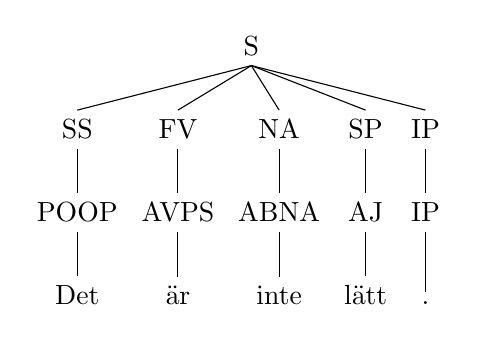
\begin{tikzpicture}
\Tree [.S [.SS [.POOP Det ]]
          [.FV [.AVPS \"ar ]]
          [.NA [.ABNA inte ] ]
          [.SP [.AJ l\"att ]]
          [.IP [.IP . ] ]
      ]
\end{tikzpicture}
}
\subfloat[Translation to GF]
{\includegraphics[width=60mm]{latt2.pdf}}
\caption{The sentence \emph{Det är inte lätt} (``It is not easy"). If the word
         \emph{lätt} (`easy') is unknown to the grammar, a meta variable is put
         in its place.}
\label{fig:gftree1}
\vspace{-5mm}
\end{figure}
between the two annotations and at the same time we get methods for extracting
and translating to GF notation. 
If a node fails to be translated, a meta variable  --annotated \verb-?- -- is put in its place.
This is also the case when two sister nodes can be translated, but no rule is
applicable for joining them into one tree.

Talbanken05 uses three kinds of tags: categories, edge labels and POS-tags. 
While the POS-tags are reserved for words, the categories give grammatical information,
such as \verb|S|, \verb|NP| and \verb|VP|.
The edge labels give the part of sentence: \verb|SS| for subject, 
\verb|OO| for object etc. 
%
%\begin{tabular}{lll}
%\textbf{Tag} & \textbf{Example} & \textbf{Explanation} \\
%\hline
%\textbf{SV} & \emph{ska} (`shall') & The verb \emph{shall}\\
%\textbf{NNDDHSGG} & \emph{familjemedlemmarnas} & Noun, definite, compound (person),\\
%&(`the family members' ') &genitive \\
%\textbf{XX} & & Unclassifiable part-of-speech\\
%\end{tabular}\\
The mapping could in some cases be performed tag-by-tag, but annotational
differences complicated the translation.
One example is valency information, which is given implicitly by the complements
of a word in Talbanken. If a verb is followed by an object, \verb-OO-, which contains an
\verb-S-, we can conclude that this is a sentence-complement verb.
In GF, the valency information is given for each entry in the lexicon.
A sentence-complement verb has the type \verb-VS- and must the 
function \verb-ComplVS- must be used for combining the verb and with a 
sentence.
%Another annotational difference that turned out to be problematic for the
%translation can be illustrated by analysis of the generic pronoun \emph{`man'}.
%In Talbanken, \emph{`man'} is simply a personal pronoun, 
%in GF it is represented by using the function \verb|GenericCl| which turns a
%\verb-VP- into a clause and has no subject visible in the abstract tree. 
%When translating a sentence like this, it is thus not possible to simply glue the
%subject to the verb with \verb|PredVP|. For each similar GF construction, an extra rule
%would be needed to get full coverage. 

%The tags \textbf{XX} and \textbf{NAC} (\verb-Not a constituent-) are often used since Talbanken makes a
%difference between subject
%and object noun phrases.
%The analysis of elliptical expression in (\ref{sent:krav})
%\enumsentence{För stora krav.\\
%``Too high demands."}\label{sent:krav}
%contains both these tags, since it is not obvious
%whether the noun phrase is used as subject or an object.
%These tags occur quite frequently in the treebank and are always translated
%to metas, which lowers our result. \\


\section{Chunk Parsing}
\label{sec:chunk}
%New section - insights about latest work
The grammar, which is hand written, cannot be expected to cover all
possible expressions of the language.
Hence, we combine it with statistical means to get good coverage. 
%The parser uses named entity recognition and a compounding analysis.
The parser should give as much output as possible 
%Further we need to be able to give output
even when encountering unknown words and grammatical constructions 
or idioms and ellipses.
Our approach makes use of the rich annotation in Talbanken -- we perform chunk parsing
relying on the tags given in the treebank. 
Consequentially, whenever a sentence is not recognized by the grammar, it is 
parsed chunk by chunk and the parse trees for each chunk is returned.
Noun phrases, adverbial phrases and adjectival phrases are considered.
Due to the differences in the annotation between Talbanken and
GF mentioned is section \ref{sec:mapping} verbs are not considered
as parsable chunks. %The GF parser depend on requires verb particles and prepositions to give
%a correct output, and which are usually not in the same Talbanken chunk. 
Therefore, our focus is on whole sentences and noun phrases. At the first stage,
we try to parse the basic sentence structure, and therefore allow the parser
to parse complicated chunks as dummy words. This way, we don't loose the 
high-level sentence analysis given by GF.
When this is done, we try to separately parse the chunks,
until as much of the sentence as possible is covered. 


%This way we get good coverage -- from ca 10 \% of Talbanken -- to ??

\section{Language Model-Based Disambiguation}

%New section - fill in with the basic principle + new results(when available)
The translation of Talbanken to GF gives us a GF treebank consisting of more than
6000 sentences. The translation process is explained in section
\ref{sec:mapping} and the trees give valuable 
information about which words from our lexicon that have been used
and which functions that are needed to parse the sentence.
GF has built-in support for probabilities, and when feeding the output
from the mapping to our grammar, we get a model of the language. 
After the parsing is completed, all trees are ranked measuring the
probability of their constituents.
As the data is extracted from manually annotated, real-world sentences,
it constitutes a reliable source for disambiguation.
%The model is used for disambiguation: the parse trees for each sentence
%are ranked by the sum of the probability of each function used.
%Both whole sentence and chunks -- phrases -- can be ranked using this
%principle.


\section{Evaluation}

For the extraction of a GF Treebank from Talbanken, (section \ref{sec:mapping})
the evaluation measures the numbers of meta variables in each translated tree.
%If the finite verb is untranslatable, we get meta variables for the verb itself and for the
%tense.
For all of Talbanken, we get a number of 65 \%, and if we limit our input to
uncomplicated sentences with no more than 10 words where all words are known to
our lexicon, we can reach 85 \%. 
%When translating the whole treebank, only 78 sentences
%could not be mapped at all and resulted in meta variables only.

%A mapping between GF and the Wall Street Journal of Penn Treebank has earlier been conducted \cite{gfMech}.
%The percentage of restored nodes from Peen Treebank is higher than our results.
%The reason for this may be the fact that English is syntactically less complicated
%than Swedish.
%Furthermore, the text in Talbanken are from various brochures, newspapers and text books,
%where idiomatic expressions are more likely the be appear and the language
%presumably less strict than in Wall Street Journal\footnote{www.wsj.com}.
%Also, the Penn Treebank contains a lower number of tags, 82 compared
%to more than 300 in Talbanken. With more tags, we get more information, but as the number 
%increase, so does the amount of work of finding the correct translation 
%for each combination of tags and writing rules that cover all constructions. \\

The evaluation of the parser is performed by testing it on Talbanken sentences
and is still being carried out. So far, our evaluation results cover
600 sentences -- about 10 \% of the treebank. 
%Without the robustness given by the chunk parser, we can only parse 17.9 \% of the sentences.
For noun phrases, we cover 76 \%.  By using the chunk parsing described in section
\ref{sec:chunk}, we identify the structure on 65 \% of the sentences. That
is, the parser can identify the verbs and how they relate to the noun phrases,
prepositions and particles. Some subtrees may  however not be
completely parsed. If a verb is unknown to the grammar, or if it is used with
another valency, other prepositions or particles than the lexicon has assigned
it, the sentence structure can not be identified. In that case
the parser returns chunks, showing the parse trees of identifiable sub-phrases.

%Section 5.3 + the evaluation part from 6.1 
%
%Latest results from chunk parsing and disambiguation



\section{Future Work}
%From 6.2 subtract the things that are already done, maybe more future
%work related to the results for chunk parsing and disambiguation. 

~~~~~~\textbf{Evaluation}
A thoroughly evaluation is still to be done. This should be carried out by
measuring the agreement between all parsed chunks and their respective
translation from Talbanken. Evaluation should also be done manually.
For this, we rely on an expert in Swedish.

%\textbf{Using the resources}
%We should make sure to make as much use of resources as possible -- Saldo,
%Talbanken and Lexin provides more information than we so far have been able to
%extract. For example, data about abbreviations and idioms should
%be added to the parser. This could be extracted from Saldo as well as Talbanken.
%As the valency information is so important to the GF grammar, the lexicon should
%be annotated with more of this in order to get a good parser.
 
\textbf{Grammar}
The grammar should cover the most prominent Swedish features.
While statistical methods compensates for constructions not covered by
the grammar, we still aim for a even wider grammar coverage. 
As examples of constructions to be added, we mention
pronominal object shift, bare indefinites and a differentiation between
object and subject control verbs.
%\vspace{-2mm}
%\begin{itemize}
%\item
%\textit{} % is common in Swedish and obligatory in Danish and Norwegian.
%\enumsentence{\begin{tabular}[t]{@{}*{11}{l@{\ }}}
%a. & Jag & ser&  honom& \textbf{inte}&~~ & b.&Jag &ser &\textbf{inte} &honom\\
%   & \emph{I} & \emph{see}&\emph{him}&\emph{not}&&& \emph{I} &\emph{see}&\emph{not}&\emph{him}\\
%\end{tabular}}
%Personal pronouns are allowed to precede negation and some other sentence adverbials % --\textit{satsadverbial} --
%in main clauses without auxiliary verbs.
%
%\enumsentence{\begin{tabular}[t]{@{}*{12}{l@{\ }}}
%a. & *Vi & har&  honom&  inte&sett&~~ & b.& * Jag &ser &huset &inte\\
%   & \emph{~we} & \emph{have}&  \emph{him}&  \emph{not} &  \emph{seen} && b.& \emph{~I}&\emph{see} &\emph{the house} &\emph{not}\\
%\end{tabular}}
%
%Although object shifts are frequently used, they are hardly found in
%Talbanken's part P, which has been the inspiration for this project.
%Therefore, this implementation has so far not been prioritized.\\

%\item
%\textit{Bare indefinites} 
%are at this point always parsed as mass nouns
%    \enumsentence{\shortexnt{3}
%{Jag & dricker& vatten}
%{\emph{I}&\emph{drink}&\emph{water}}
%}\label{sent:water}
%although this clearly is a unsatisfying analysis for bare indefinites as in (\ref{sent:hund})
%\enumsentence{\shortex{4}
%{Vi & ska& köpa & hund}
%{\emph{we} &\emph{will}& \emph{buy} & \emph{dog} }
%{``We are going to buy a dog"}}\label{sent:hund}
%\vspace{3mm}

%\item
%\textit{Object and subject control verbs}
%It should for example be possible to differentiate between 
%object and subject control verbs.
%
%\eenumsentence{
%\item[a]\shortex{7}
%{Han & ber & henne & att & städa & sitt & rum}
%{\emph{he} & \emph{begs} & \emph{her} & \emph{to} & \emph{clean} & {\sc self's} & \emph{room}}
%{``He asks her to clean her room"}
%\item[b]\shortex{7}
%{Han& lovar& henne& att& städa &sitt & rum}
%{\emph{he}& \emph{promises}& \emph{her}& \emph{to}&  \emph{clean} &\sc self's&\emph{room}}
%{``He promises her to clean his room"}}
%\end{itemize}


\textbf{Improving memory and time consumption}
When using GF for parsing with lexicon of our size, we currently
suffer from memory usage problems. The parsing algorithm is not fully
capable of evaluating all possible parse trees, which is necessary in order
to find the best one.

%\textbf{Dealing with valency information}
%Many Swedish verbs can be used with different number of arguments.
%Having one lexical entry for every possible usage of a verb
%does not seem to be a good idea considering
%the ambiguities it will lead to and the already high time usage.
%Still valencies is crucial when parsing, and methods for handling 
%this within the robust layer of the parser are to be implemented, possibly
%implemented by using external resources.



\section{Conclusion}
%From 6.1 - the discussion part + something about the latest work
Our work resulted in a wide-coverage grammar for Swedish which --
combined with statistical resources -- can be used for parsing 
open-domain text. The grammar covers a large number of syntactic 
phenomena and uses an extensive morphological lexicon. To
our knowledge, it is the most comprehensive computational grammar for
Swedish and the most complex GF grammar to date.
Besides parsing, the grammar may well be used for language generation.

All parts of the project is open-source and the grammar and other parts
are modular and may well be reused and developed.

%Open source, transparent, modular, explores the strengths and weakneses
%of GF.
\bibliographystyle{splncs}
\bibliography{FinBib}

\end{document}
